% PICOCON 37 information booklet, 2020.
\documentclass[12pt]{article}
\usepackage[a4paper,bottom=2.5cm,left=2cm,right=2cm,top=2cm]{geometry}

%paragraph spacing
\usepackage{parskip}
\setlength{\parskip}{1em}
\makeatletter
\newcommand{\@minipagerestore}{\setlength{\parskip}{1em}}
\makeatother

%hyphenation, date format, font encoding
\usepackage[british]{babel}
\usepackage[condensed]{roboto}
\usepackage{tgtermes}
\usepackage[T1]{fontenc}

% UTF input
\usepackage[utf8]{inputenc}

% dagger footnotes & re-start count every page
\usepackage{perpage}
\MakePerPage[2]{footnote}
\renewcommand{\thefootnote}{\fnsymbol{footnote}}

% graphics imports
\usepackage{graphicx}

\usepackage{caption}

% timetable formatting
\usepackage{array}
\usepackage{multirow}

% end mark
\newcommand{\tombstone}[1]{%
  \includegraphics[height=\fontcharht\font`\B,clip]{#1}%
}

\newcommand{\altf}[1]{\textsf{\textbf{\uppercase{#1}}}}

% page header
\newcommand{\head}[1]{%
  \begin{center}
    {\Huge\altf{\textbullet{} #1 \textbullet{}}}
  \end{center}%
}
\newcommand{\subhead}[1]{%
  {\Large\altf{#1}\par}%
}



\begin{document}
%
% \thispagestyle{empty}
% \begin{center}
%     % 
\includegraphics[width=\textwidth]{img/profile/placeholder.png}
%     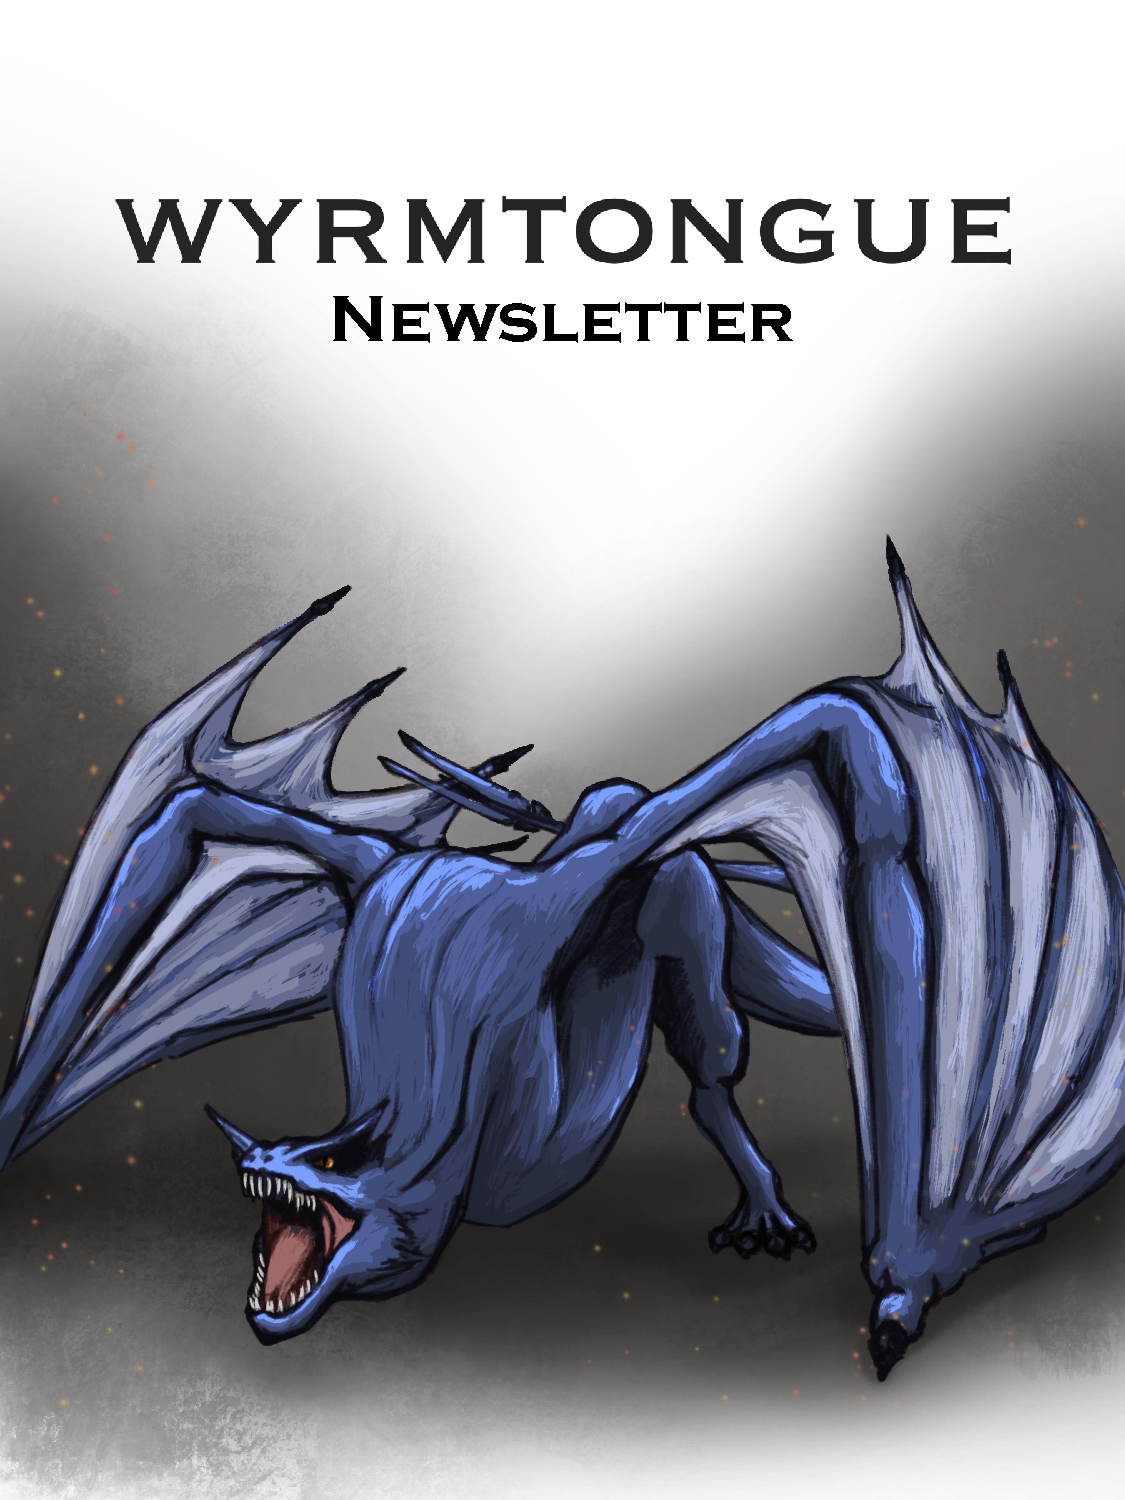
\includegraphics[width=\linewidth]{img/newsletter-cover-no-logo-2024.pdf}
% \end{center}
% \par\vspace{\fill}
% \begin{center}
%   
\includegraphics[width=0.4\textwidth]{img/logo/logo-alt.png}
% \end{center}

\begin{titlepage}
    \AddToShipoutPictureBG*{%
              \AtPageLowerLeft{%
                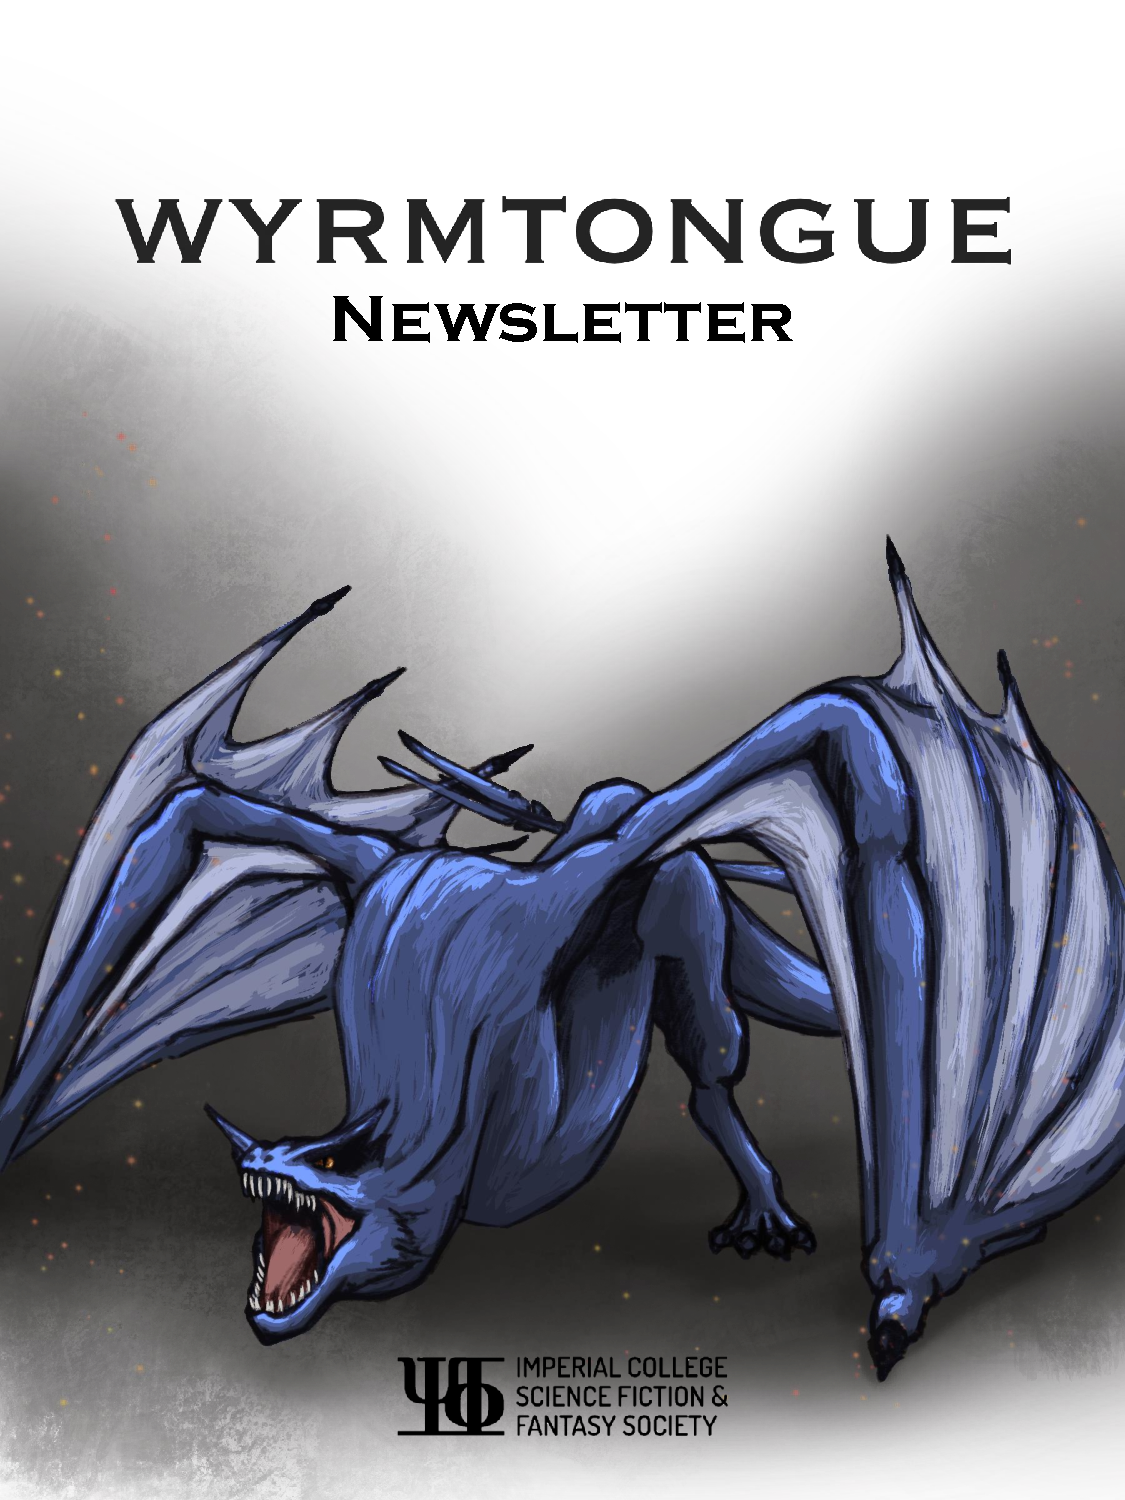
\includegraphics[width=\paperwidth,height=\paperheight]{img/newsletter-cover-2024.pdf}%
              }%
            }
\end{titlepage}

\textbf{      } % this is so hacky

\clearpage
%
\head{The King's Speech}
\clearpage
%
\head{The Sofa's Ramblings}
\clearpage
%
\head{A Word from the Beanbag}
\clearpage
%
\head{Schedule}
\newcommand{\scheduleitem}[2]{%
  \multirow{#1}{*}{
    \begin{minipage}[t]{0.7\textwidth}
      #2
    \end{minipage}
  }%
}
\newcommand{\at}[1]{\hfill{\footnotesize #1}}

\begin{center}
  \renewcommand{\arraystretch}{2.2}
  \begin{tabular}[t]{>{\ttfamily}r l}
    10:00 & front desk / registration opens \\\hline
    10:30 & \scheduleitem{2}{
      Guest Talk: \textbf{Roz Kaveney}
      \at{Blackett Building LT1}
    } \\
    11:00 \\
    \hline
    11:30 & \scheduleitem{2}{
      Guest Talk: \textbf{Tamsyn Muir}
      \at{Blackett Building LT1}
    } \\
    12:00 \\
    \hline
    12:30 & \scheduleitem{3}{
      \textbf{Lunch}
      \vspace{1em}\newline
      \textbf{Intro Lightsabre Session}
      \at{Location?}
    } \\
    13:00 \\
    13:30 \\
    \hline
    14:00 & \scheduleitem{2}{
      Guest Talk: \textbf{Juliet Kemp}
      \at{Blackett Building LT1}
    } \\
    14:30 \\
    \hline
    15:00 & \scheduleitem{2}{
      \textbf{Group Panel}
      \at{Blackett Building LT1}
    } \\
    15:30 \\
    \hline
    16:00 & \scheduleitem{5}{
      \textbf{Destruction of Dodgy Merchandise}
      \at{Queen's Lawn 16:00 -- 16:30}
      \vspace{1em}\newline
      \textbf{Charity + Silly Games}
      \at{Blackett Building LT1}    
    } \\
    16:30 \\
    17:00 \\
    17:30 \\
    18:00 \\
    \hline
    18:30 & \textbf{Harmless Fun} \footnotemark \at{Queen's Lawn} \\
    \hline
    19:00 & \scheduleitem{2}{
      \textbf{Pub Quiz}
      \at{Location?}
    } \\
    19:30 \\
  \end{tabular}
\end{center}

\footnotetext{definitely not a fish duel.}

\clearpage
%
\head{Guests of Honour}
\newcommand{\profiletxt}[1]{
  \begin{minipage}[t]{0.74\textwidth}
    \vspace{0pt}
    \input{#1}
  \end{minipage}
}
\newcommand{\profileimg}[2]{
  \begin{minipage}[t]{0.22\textwidth}
    \vspace{0pt}
    \includegraphics[width=\textwidth]{#2}
    \\ [0.5em]
       {\Large \altfont{#1}}
  \end{minipage}
}
\newcommand{\profile}[3]{
  \checkoddpage\ifoddpage
  \profiletxt{#3}\hspace*{\fill}\profileimg{#1}{#2}
  \else
  \profileimg{#1}{#2}\hspace*{\fill}\profiletxt{#3}
  \fi
}
%% \newcommand{\profile}[3]{
%%   % #1 - name
%%   % #2 - path to image
%%   % #3 - path to text
%%   \begin{minipage}[t]{0.74\textwidth}
%%     \vspace{0pt}
%%     \input{#3}
%%   \end{minipage}
%%   \hspace*{\fill}
%%   \begin{minipage}[t]{0.22\textwidth}
%%     \vspace{0pt}
%%     \includegraphics[width=\textwidth]{#2}
%%     \\ [0.5em]
%%     {\Large \altfont{#1}}
%%   \end{minipage}
%% }%
\profile{Brendan Dubois}
        {img/guests/b-dubois.jpg}
        {txt/guests/d-dubois}

\profile{A.J. Flowers}
        {img/guests/a-flowers.jpg}
        {txt/guests/a-flowers}
        
\profile{Louise Mumford}
        {img/guests/l-mumford.jpg}
        {txt/guests/l-mumford}
\profile{Bryony Pearce}
        {img/guests/b-pearce.jpg}
        {txt/guests/b-pearce}
        
\profile{Gareth Powell}
        {img/guests/g-powell.jpeg}
        {txt/guests/g-powell}
        
\profile{Matthew Wraith}
        {img/guests/m-wraith.jpg}
        {txt/guests/m-wraith}

\clearpage
%
\head{Tabletop\&Gaming}
\vfill
\head{Vendors}
Our vendors are located on the second floor of the Blackett foyer, and and would love to introduce themselves to you.

\vspace{5mm}

{\Large Paul Couper}

A reader/collector of SF/Fantasy, selling at Picocon to clear duplicates built up whilst collecting and upgrading. My collection is now over 12,000 paperbacks, but still has many gaps. Most wanted at present? Probably E Pluribus Unicorn, Theodore Sturgeon, Timescape paperback (i.e. 4th Pocket printing) to complete my timescape collection. So if anyone has a copy of that (or other collectables) for sale, wants to buy, or indeed just wants a chat, stop by during the day.

\vspace{5mm}

{\Large Clockwork Firebird Designs - Alex Locke }

Welcome to Clockwork Firebird Designs! I am a self-taught, ever-evolving tailor, leather worker and costume maker with a penchant for creating monsters. I attend Live Action Role-Play (LARP) events and Anime/Comic conventions as both a trader and attendee on a regular basis. I've been doing leather work since 2008, and selling since 2011. I recall learning to sew when I was 6 years old and I've not really stopped since. Within the shop you may find armour, masks, trinkets, painted artworks, soft toys... anything I bring to mind or feel like turning my hand to! I am still finding my feet, and I am always learning new techniques.

\vspace{5mm}

{\Large Blackwell Books }

This year, giving you an even greater selection of books to browse from, we will also be welcoming Blackwell's for the first time. For Picocon, they will primarily be stocking books by our Guests of Honour, so it will be a great chance for you to grab a copy of the books you've heard all about today!
\vfill
\clearpage
\end{document}
